\chapter{Implementation: Incremental detection}
\label{dynamicdetection}

The following chapter will present the algorithm which efficiently updates the list of
clones, without having to rebuild the different structures from scratch. Given an edit
to a file in the project, we will be able to update the document index, fingerprints,
suffix array and list of clones faster than the initial detection.

An incremental update is run whenever a document is changed. The document index is
signalized of a change either when a file is saved, or on any keystroke. This is
configurable by the client. When the document index is changed, an incremental update of
the clones is run, and the clone-list is updated.

\section{Affordable operations}

Before looking at the approach, it is useful to determine the time cost associated with
different operations. We can for example afford to iterate over the contents of a
single file, which will be useful for our algorithm. 

We cannot afford to iterate over the entire code base, meaning the contents of all files
in the code base. The initial detection takes linear time in the size of the code base,
therefore, iterating over the entire code base will likely make the algorithm as slow as
the initial detection. The same goes for the iterating over the entire fingerprint.

As mentioned, we can afford to iterate over the contents of a single file. Iterating over
the contents of a file with up to a few thousands lines is not a very expensive operation
to perform and will not take a significant amount of time. The whole string of the file
contents will be needed for Tree-sitter to incrementally parse the file.

Parsing an entire file however, can be too expensive in some cases. While the runtime of
parsing a single file is still linear in the size of file content, parsing a large file
from scratch can take a significant amount of time in practice, and for small code bases
with large files, parsing can take a significant portion of the total runtime of a dynamic
update. This is why incremental parsing with Tree-sitter is used, which lowers the runtime
closer to $O(\vert\text{edit}\vert)$, rather than $O(\vert \text{file} \vert)$

We can also afford two more useful operations, iterating over the documents in the index
(not their contents), and iterating over the clone objects. We can afford to do these
operations because the number of documents and the number of clones is likely multiple
magnitudes lower than the size of the entire code base. Iterating over the documents
will be useful when we are updating the document index, and iterating over the clones is
necessary to do when the clones are mapped back to their original source code locations.

Why we can afford these operations will be become clearer in \cref{evaluation}, the main
idea is that all the operations we can afford will take an insignificant amount of time
compared to updating the suffix array.

\section{Updating the document index}

\begin{figure}[H]
    \begin{center}
        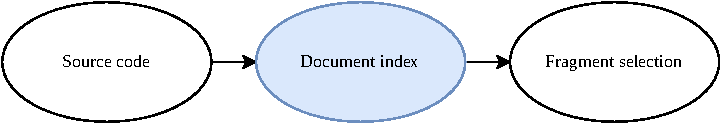
\includegraphics[width=0.8\textwidth]{figures/phases/phases_documentindex.drawio.pdf}
    \end{center}
\end{figure}

The first step of an incremental update is to update the document index. We will also look
at how we can reduce the memory usage of the index without a loss in terms of the time
complexity of the updates.

As previously shown, each document stores its own content, AST and fingerprint. It is not
strictly necessary to store either the content or the AST in memory all the time, as it is
likely that only a handful of files are open in the IDE at once. Therefore, in the initial
detection, we can free the memory of the file content and AST for each document after the
fingerprint has been computed. However, if a file is opened in the IDE, the file can now
be changed, so we should facilitate efficient updates for these files at least. When a
file is opened, the file content should be read from the disk and updated via the
\verb|textDocument/didChange| messages sent from the client. It is also important to keep
the AST of the opened file in memory in order to facilitate incremental parsing of the
opened files. 

When a file is opened, the LSP client sends a \verb|textDocument/didOpen| message to the
server, which finds the relevant document $D$ in the index, and sets the following fields:

\begin{flalign*}
&\Access{D}{\Var{open}} = \True \\
&\Access{D}{\Var{content}} = \Read{$\Access{D}{\Var{uri}}$} \\
&\Access{D}{\Var{AST}} = \Parse{$\Access{D}{\Var{content}}$}
\end{flalign*}

After the document fields have been set, the document is ready to receive updates. When
the LSP client sends a \verb|textDocument/didChange| message, the message consists of the
URI of the edited file, the range of the content which has changed, and the content which
has potentially been inserted. This range is then used in a tree-sitter incremental parse
of the file content. After this parse, we have efficiently updated a documents content and
AST. After this update, we also set $\Access{D}{\Var{changed}} = \True$

\section{Updating fingerprints}

\begin{figure}[H]
    \begin{center}
        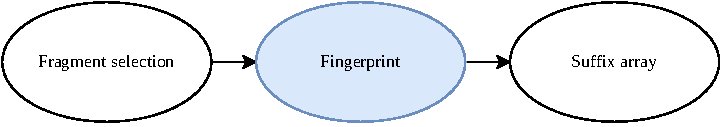
\includegraphics[width=0.8\textwidth]{figures/phases/phases_fingerprint.drawio.pdf}
    \end{center}
\end{figure}

With the updated AST for all documents, we can update the fingerprint of all documents
which have been changed. For each document $D$ where $\Access{D}{\Var{changed}} = \True$,
the fingerprint for $D$ may have changed. Computing the new fingerprint is the same
process as in the initial detection, where we first query the AST for all nodes of a
certain type, then for each matched node $N$, we extract and fingerprint all the tokens
which $N$ covers, using the same fingerprint mapping as was used for the initial
detection.

An additional change we have to consider when incrementally updating fingerprints is that
for a document $D$, $\Access{D}{start}$ and $\Access{D}{end}$ which corresponds to the
range which $D$ covers in the fingerprint, may have changed.  Also, any document $D_1$
where $\Access{D_1}{start} > \Access{D}{start}$ could also have its range changed. This
range needs to be updated in order for the source-mapping to work. This is solved while
updating each documents fingerprint by counting the number of tokens in each document
after updating, and setting the appropriate \verb|start| and \verb|end| fields.

Figure \ref{fig:fingerprintupdate} shows how an index of three documents is updated when
two tokens are inserted. Note that each document stores its own fingerprint, we do not
need to concatenate them to one large array as in the initial detection.

\begin{figure}[t]
    \begin{center}
        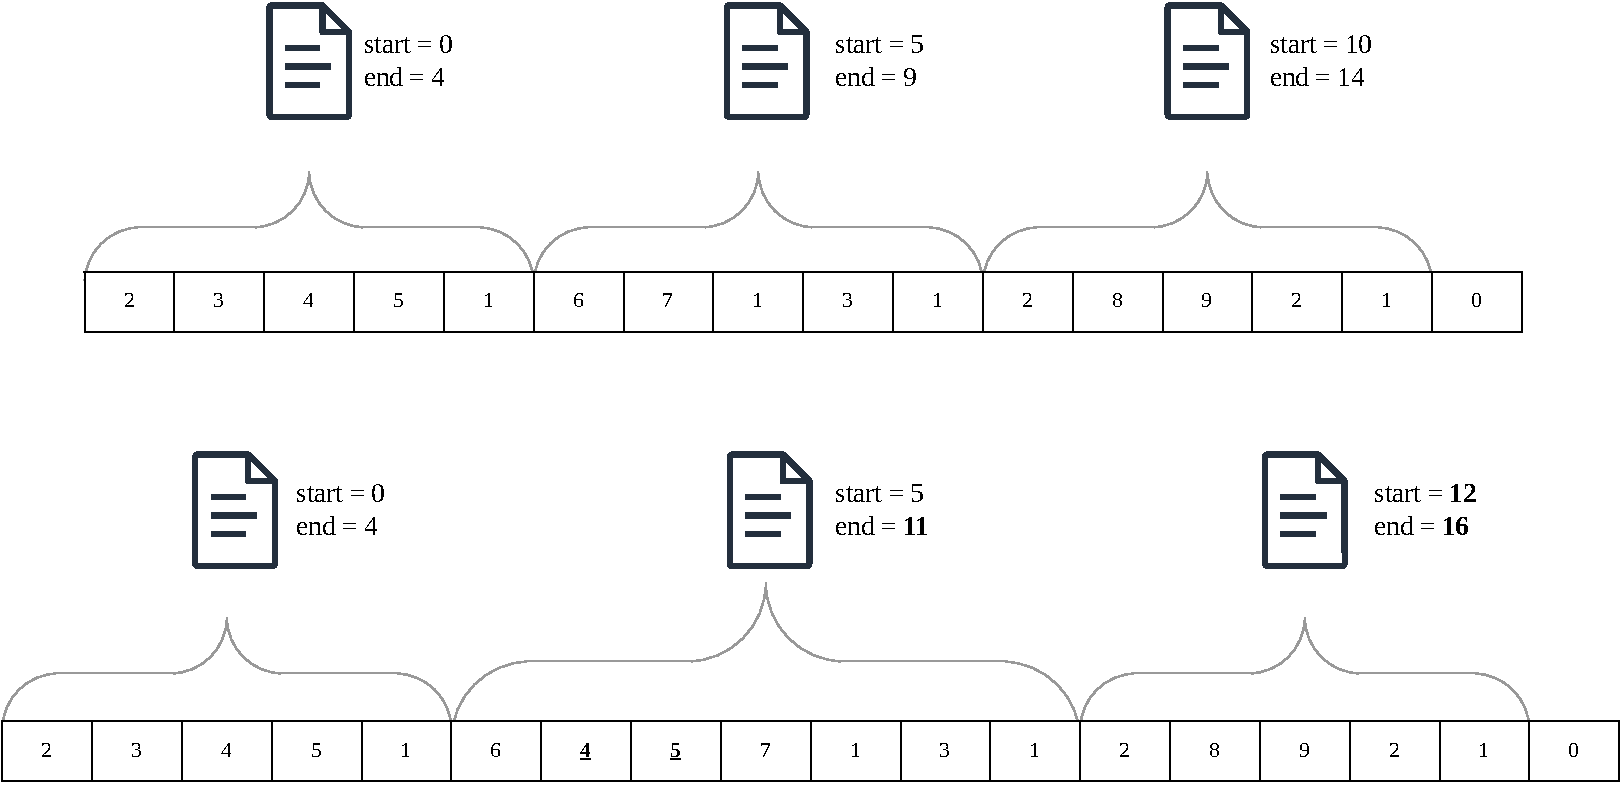
\includegraphics[width=0.95\textwidth]{figures/indexupdate.drawio.pdf}
    \end{center}
    \caption{Old (above) and new (below) fingerprints and ranges when two tokens are inserted}
    \label{fig:fingerprintupdate}
\end{figure}

\section{Computing edit operations}

Now that the fingerprint has been updated, we could build the suffix array from scratch
and already see a substantial improvement in performance. The major bottleneck of the
initial detection is to parse and fingerprint the entire code base. Instead, we want to
further improve the efficiency by dynamically updating the suffix array.

The input to the dynamic suffix array algorithm is a set of edit operations. An edit
operation can be either deleting, inserting or substituting a set of consecutive
characters in the fingerprint. The dynamic suffix array algorithm will take each edit
operation, and update its suffix array to reflect the new state of the fingerprint.
Therefore, the first problem to solve is to determine what exactly has changed in the
fingerprint. 

There are a couple of approaches we could take to determine the edit operations. The
simplest is that whenever a file has changed, regard the entire file as changed, and
perform a delete operation which removes the entire fingerprint of that file, and then an
insertion which inserts the new fingerprint of that file. This is a very simple approach,
but can lead to an unnecessary size for the edit operations. The fingerprint of the file
is likely to be very similar to the previous version, therefore deleting and then
inserting the entire files fingerprint could be a lot more work than it needs to be.
However, this idea that we can always reduce the number of operations to only two, a
deletion and an insertion, will be useful in our final algorithm.

Another possible approach is to look at the ranges that the LSP client provides with each
\verb|textDocument/didChange| message and determine which tokens in the fingerprint have
been affected according to this range. However, this approach tightly couples the
algorithm to LSP and the scenario where we know the exact ranges of each change. Also, we
might do unnecessary amounts of operations if we do multiple edits, since some operations
could cancel each other out, for example by inserting and then deleting the same text.

A better approach is to determine the changes of the fingerprint using an edit distance
algorithm. An edit distance algorithm is an algorithm which computes the distance between
two strings $S_1$ and $S_2$. Distance between two strings is the minimum number of edit
operations (insert, delete, substitute) which is required to transform $S_1$ into $S_2$.
Many of the algorithms which computes the edit distance, also allows computing what the
operations are.

The classic algorithm for calculating edit distance operations is attributed to Wagner and
Fischer~\cite{WagnerFischer}. The input to the algorithm is two strings $S_1$ and $S_2$ of
length $n$ and $m$. The output will be the set of operations needed to turn $S_1$ into
$S_2$. This algorithm is based on dynamic programming where a matrix $M$ is filled from
top to bottom and then the operations are inferred from $M$. The recurrence in equation
\ref{eq:editdistancerecurrence} shows how the edit distance matrix is filled and
\ref{tab:wagnerfischermatrix} shows an example matrix.

\begin{figure}[t]
    \begin{center}
	$$
		\sum^{n}_{i = 0}{M[i][0] = i}
	$$
	$$
		\sum^{m}_{j = 0}{M[0][j] = j}
	$$

	\begin{gather*}
		M[i][j] =
		\begin{cases}
			M[i-1][j-1] & \mathrm{if\ } S_1[i] = S_2[j] \\
            1 + \Min{$M[i-1][j-1], M[i][j-1], M[i-1][j]$}
		\end{cases}
	\end{gather*}
	\caption{Edit distance recurrence}
	\label{eq:editdistancerecurrence}
    \end{center}
\end{figure}

Each index $i, j$ in $M$ contains the edit distance value between the substrings
$\ArrayAccess{S_1}{0..i}$ and $\ArrayAccess{S_2}{0..j}$ The values in $M$ is calculated by
determining what is the cheapest operation to do at a certain location to make the
substrings equal. This can be determined by looking at the three surrounding indices in
$M$: $\MatrixAccess{M}{i - 1}{j - 1}$, $\MatrixAccess{M}{i - 1}{j}$ and
$\MatrixAccess{M}{i}{j - 1}$. Each of these indices equate to deleting, inserting or
substituting a character in $S_1$. 

\begin{table}
	\begin{center}
		\begin{tabular}[c]{c|c|c|c|c|c|c|c|c|c|}
			  &                      & D                    & E                    & M                    & O                    & C                    & R                    & A                    & T                    \\\hline
			  & \cellcolor{blue!25}0 & 1                    & 2                    & 3                    & 4                    & 5                    & 6                    & 7                    & 8                    \\\hline
			R & 1                    & \cellcolor{blue!25}1 & 2                    & 3                    & 4                    & 5                    & 5                    & 6                    & 7                    \\\hline
			E & 2                    & 2                    & \cellcolor{blue!25}1 & 2                    & 3                    & 4                    & 5                    & 6                    & 7                    \\\hline
			P & 3                    & 3                    & \cellcolor{blue!25}2 & 2                    & 3                    & 4                    & 5                    & 6                    & 7                    \\\hline
			U & 4                    & 4                    & \cellcolor{blue!25}3 & 3                    & 3                    & 4                    & 5                    & 6                    & 7                    \\\hline
			B & 5                    & 5                    & 4                    & \cellcolor{blue!25}4 & 4                    & 4                    & 5                    & 6                    & 7                    \\\hline
			L & 6                    & 6                    & 5                    & 5                    & \cellcolor{blue!25}5 & 5                    & 5                    & 6                    & 7                    \\\hline
			I & 7                    & 7                    & 6                    & 6                    & 6                    & \cellcolor{blue!25}6 & 6                    & 6                    & 7                    \\\hline
			C & 8                    & 8                    & 7                    & 7                    & 7                    & 6                    & \cellcolor{blue!25}7 & 7                    & 7                    \\\hline
			A & 9                    & 9                    & 8                    & 8                    & 8                    & 7                    & 7                    & \cellcolor{blue!25}7 & 8                    \\\hline
			N & 10                   & 10                   & 9                    & 9                    & 9                    & 8                    & 8                    & 8                    & \cellcolor{blue!25}8 \\\hline

			\hline
		\end{tabular}
	\end{center}
	\caption{Edit distance matrix for REPUBLICAN $\rightarrow$ DEMOCRAT}
	\label{tab:wagnerfischermatrix}
\end{table}


The edit operations can then be inferred from $M$ by backtracking from the bottom-right
index, to the top-left, giving us the edit operations in reverse. At each position $i, j$
we choose either of the 3 surrounding indices, the same indices which were used to
determine the value originally. Choosing the left index ($i, j - 1$) equates to inserting
the character $\ArrayAccess{S_2}{j - 1}$ at position $i - 1$. Choosing the top index ($i -
1, j$) equates to deleting the character $\ArrayAccess{S_1}{i - 1}$. Choosing the top-left
index ($i - 1, j - 1$) equates to substituting $\ArrayAccess{S_1}{i - 1}$ with
$\ArrayAccess{S_2}{j - 1}$. If these characters are already equal, the operation can be
ignored. For example in table \ref{tab:wagnerfischermatrix}, the first operation is to
substitute \verb|R| with \verb|D| at position $0$. Afterwards \verb|P| and \verb|U| is
deleted at position $2$. Then the \verb|B| which is now at position $2$ is substituted by
\verb|M|. This continues with more substitutions until we finally have \verb|DEMOCRAT|.

\subsection*{Aggregating edit operations}

In the next phase we will feed the edit operations into an algorithm which dynamically
updates our suffix array based on those operations. However, this algorithm will be more
efficient if the operations are combined to singular inserts, deletes or substitutes of
strings more than one character. The edit distance algorithm outputs only single character
operations, meaning we insert, delete or substitute a single character at a time. We
therefore want a way to combine these operations to ``larger'' operations.

We define an EditOperation with the following record:

\begin{lstlisting}
EditOperation {
    OperationType type,
    char[] chars,
    int position
}
\end{lstlisting}

where type is either an insert, delete or substitute.

One way to combine operations is to find operations of the same type which are sequenced
in the matrix. For example in table \ref{tab:wagnerfischermatrix}, we have two consecutive
delete operations, where \verb|P| and \verb|U| is deleted at position $2$. These two
operations could be combined to a single delete operation of two characters.

The idea for the algorithm which computes the edit operations is to traverse the optimal
matrix path backwards and for each operation we either append to the current operation if
possible, or start a new operation. We can continue the current operation if the next
operation is of the same type, and the next operation has the same position as the current
operation. For example in table \ref{tab:wagnerfischermatrix}, we have two delete
operations in a sequence at position $1$ where \verb|P| and \verb|U| is deleted. The first
operation we encounter is the deletion of \verb|U|. At this point we create a new
\verb|EditOperation| with position $1$ and \verb|U| in the \verb|chars| array. The next
operation is also a delete operation at position $1$, so we add the \verb|P| to the list
of characters for the operation to delete. The next operation is a substitute at position
$0$, so we cannot continue the delete operation, and a new substitute operation is created
instead. Similarly, at position $2$ to $5$, we substitute \verb|BLIC| with \verb|MOCR|.
This operation is computed in a backwards fashion similarly to how we did the deletion,
except that the position of the operation is decremented for each character we add to it.

Note that this algorithm is not an optimal algorithm, as this is a trade-off between
processing many characters in few operations, versus processing many operations with few
characters. As mentioned earlier, one could always reduce the solution to be only two
operations, deleting the whole string, and inserting the new string. This is only two
operations, but likely processes more characters in total compared to our algorithm. 

\subsection*{Optimizing memory usage and operations}

A problem with the above solution is the memory usage of the matrix. It is not feasible to
input the entire old and new fingerprint into an edit distance algorithm, as the full
fingerprint can have millions of symbols, and the old and new fingerprint is likely
approximately the same size. This would require a matrix which is too large to fit in
memory. We will use a few techniques to reduce the memory usage of this algorithm without
compromising on the time complexity.

The first technique is to not input the whole fingerprint. We can drastically reduce the
size of the input by only comparing the old and new fingerprint of the document $D$ which
has been edited. $D$ stores its previous and current fingerprint, and whenever it is
edited, we can compute the edit operations of $D$, with its previous and current
fingerprint as input. However, the position of each edit operation of $D$ will not have
the correct position relative to the entire fingerprint, so $\Access{D}{start}$ is
added to the position of each edit operation to correct this.

Another optimization we can do to reduce the size of the matrix is to remove the
``trivial'' part at each end of our matrix. If we compare two strings which have many
similar characters at the beginning or end of our string, we know that these will not
produce any edit operations in the matrix, as they will simply be diagonal moves
(substitutes) where the characters are already equal. In table
\ref{tab:minimizededitmatrix} we see the edit matrix for the input \verb|FASCINATING| and
\verb|FINISHING|. The two words share the common prefix \verb|F| and the common suffix
\verb|ING|. If we examine the edit distance values, we see that the highlighted green
matrix starts at $0$ in the top left, and ends with $6$ in the top right, which is the
same final values as in the full matrix. Also, we see that there are no edit operations
being added outside the green matrix. Using this knowledge, we can see that we only need
to compare the strings \verb|ASCINAT| and \verb|INISH|, which would give us the exact same
edit distance. We can also get the exact same edit operations, as long as we account for
the starting offset of the original string, so that the operations have the correct
positions. Algorithm \ref{alg:minimizededitstrings} shows how two input strings can be
minimized for usage in the edit distance algorithm. After getting the edit operations from
the algorithm, the \verb|startOffset| is added to the position of each operation to
account for the offset of the minimized matrix.

\begin{table}
	\begin{center}
		\begin{tabular}[c]{c|c|c|c|c|c|c|c|c|c|c|}
			  &                      & F                     & I                     & N                     & I                     & S                     & H                     & I                    & N                    & G                    \\\hline
			  & \cellcolor{blue!25}0 & 1                     & 2                     & 3                     & 4                     & 5                     & 6                     & 7                    & 8                    & 9                    \\\hline
			F & 1                    & \cellcolor{blue!25}0  & \cellcolor{green!25}1 & \cellcolor{green!25}2 & \cellcolor{green!25}3 & \cellcolor{green!25}4 & \cellcolor{green!25}5 & 6                    & 7                    & 8                    \\\hline
			A & 2                    & \cellcolor{green!25}1 & \cellcolor{blue!25}1  & \cellcolor{green!25}2 & \cellcolor{green!25}3 & \cellcolor{green!25}4 & \cellcolor{green!25}5 & 6                    & 7                    & 8                    \\\hline
			S & 3                    & \cellcolor{green!25}2 & \cellcolor{green!25}2 & \cellcolor{blue!25}2  & \cellcolor{green!25}3 & \cellcolor{green!25}3 & \cellcolor{green!25}4 & 5                    & 6                    & 7                    \\\hline
			C & 4                    & \cellcolor{green!25}3 & \cellcolor{green!25}3 & \cellcolor{blue!25}3  & \cellcolor{green!25}3 & \cellcolor{green!25}4 & \cellcolor{green!25}4 & 5                    & 6                    & 7                    \\\hline
			I & 5                    & \cellcolor{green!25}4 & \cellcolor{green!25}3 & \cellcolor{green!25}4 & \cellcolor{blue!25}3  & \cellcolor{green!25}4 & \cellcolor{green!25}5 & 4                    & 5                    & 6                    \\\hline
			N & 6                    & \cellcolor{green!25}5 & \cellcolor{green!25}4 & \cellcolor{green!25}3 & \cellcolor{green!25}4 & \cellcolor{blue!25}4  & \cellcolor{green!25}5 & 5                    & 4                    & 5                    \\\hline
			A & 7                    & \cellcolor{green!25}6 & \cellcolor{green!25}5 & \cellcolor{green!25}4 & \cellcolor{green!25}4 & \cellcolor{green!25}5 & \cellcolor{blue!25}5  & 6                    & 5                    & 5                    \\\hline
			T & 8                    & \cellcolor{green!25}7 & \cellcolor{green!25}6 & \cellcolor{green!25}5 & \cellcolor{green!25}5 & \cellcolor{green!25}5 & \cellcolor{blue!25}6  & 6                    & 6                    & 6                    \\\hline
			I & 9                    & 8                     & 7                     & 6                     & 5                     & 6                     & 6                     & \cellcolor{blue!25}6 & 7                    & 7                    \\\hline
			N & 10                   & 9                     & 8                     & 7                     & 6                     & 6                     & 7                     & 7                    & \cellcolor{blue!25}6 & 7                    \\\hline
			G & 11                   & 10                    & 9                     & 8                     & 7                     & 7                     & 7                     & 8                    & 7                    & \cellcolor{blue!25}6 \\\hline \end{tabular} \end{center} \caption{Edit distance matrix for FASCINATING $\rightarrow$ FINISHING. Blue
		is optimal path, green is minimized matrix}
	\label{tab:minimizededitmatrix}
\end{table}

\begin{algorithm}[t]
  \SetAlgoLined\DontPrintSemicolon
    \algo{\EditDistanceMinimizeStrings{$S_1$, $S_2$}}{

        \For{$i \From 0 \To \Min{$\Len{$\Var{S}_1$}, \Len{$\Var{S}_1$}$}$}{
            \lIf{$\ArrayAccess{\Var{S_1}}{\Var{i}} \neq \ArrayAccess{\Var{S_2}}{\Var{i}}$}{
                \Break
            }
        }
        $\Var{startOffset} \gets i$ \;\;


        $\Var{s1End} \gets \Len{$\Var{S}_1$} - 1$ \;
        $\Var{s2End} \gets \Len{$\Var{S}_2$} - 1$ \;

        \While{$\Var{s1End} \geq \Var{startOffset} \And \Var{s2End} \geq
        \Var{startOffset} \And \ArrayAccess{\Var{S_1}}{\Var{s1End}} =
        \ArrayAccess{\Var{S_2}}{\Var{s2End}}$}{
            $\Var{s1End} \gets \Var{s1End} - 1$ \;
            $\Var{s2End} \gets \Var{s2End} - 1$ \;
        } \;

        $\Var{miniS1} \gets \ArrayAccess{\Var{S}_1}{\Var{startOffset}...\Var{s1End}}$ \;
        $\Var{miniS2} \gets \ArrayAccess{\Var{S}_2}{\Var{startOffset}...\Var{s2End}}$ \;\;

        \Return{$(\Var{miniS1}, \Var{miniS2}, \Var{startOffset})$}
    }

  \vspace{0.5cm}
  \caption{Minimize strings for edit distance algorithm}
  \label{alg:minimizededitstrings}
\end{algorithm}

The two optimizations drastically reduce the memory and time usage of the edit distance
algorithm, but in cases where a very large file is edited, and the beginning and end of
the old and new fingerprint do not match, we can still encounter instances of the matrix
being too large to fit in memory. The problem is that the matrix size has a polynomial
growth in terms of the fingerprint size. This is because the old fingerprint is of size
$n$ and the new fingerprint is of size $m$, where $n \approx m$, which requires an $n
\times m$ size matrix to calculate the edit operations. For example if a Java file
contains $3000$ lines, the number of tokens can exceed $10000$, which would require
approximately a $10000^2$ size matrix, which is approaching a memory usage which too
large.

A solution to this problem is to reduce the required memory from the polinomial $O(n \times m)$
memory usage, to a linear $O(n)$ memory usage. A stepping stone towards such a solution is
an observation attributed to Ukkonen, which reduces the required memory to linear growth
in the size of either of the strings~\cite{UkkonenEditDistance}. The observation shows
that in order to compute the next row/column of the edit distance matrix, we only need the
previous row/column. For example in table \ref{tab:minimalmemoryusageeditdistance}, the
fifth row has been computed using only the fourth row. This is done by first computing the
left-most index of the fifth row, which is always one more than the previous row.
Afterwards, we can compute the other elements of the row from left to right, with the same
recurrence, shown in equation \ref{eq:editdistancerecurrence}. This is possible because we
always know the above, left, and top-left elements of the current index. This can be
implemented as two arrays, which holds the previous and current row. 

\begin{table}[t]
	\begin{center}
		\begin{tabular}[c]{c|c|c|c|c|c|c|c|c|c|}
			  &   & D & E & M & O & C & R & A & T \\\hline
			  &   &   &   &   &   &   &   &   &   \\\hline
			R &   &   &   &   &   &   &   &   &   \\\hline
			E &   &   &   &   &   &   &   &   &   \\\hline
			P & 3 & 3 & 2 & 2 & 3 & 4 & 5 & 6 & 7 \\\hline
			U & 4 & 4 & 3 & 3 & 3 & 4 & 5 & 6 & 7 \\\hline
			B &   &   &   &   &   &   &   &   &   \\\hline
			L &   &   &   &   &   &   &   &   &   \\\hline
			I &   &   &   &   &   &   &   &   &   \\\hline
			C &   &   &   &   &   &   &   &   &   \\\hline
			A &   &   &   &   &   &   &   &   &   \\\hline
			N &   &   &   &   &   &   &   &   &   \\\hline
		\end{tabular}
	\end{center}
	\caption{Edit distance matrix with minimal memory usage}
	\label{tab:minimalmemoryusageeditdistance}
\end{table}

This change allows us to compute the edit distance in linear space, but now the problem is
how to find the actual edit operation. This is not possible, because we don't have the
entire matrix available to traverse anymore. However, this can be solved using
Hirschberg's algorithm~\cite{HirschbergsAlgorithm}. Hirschberg's algorithm is an algorithm
which can compute the edit operations of two strings in the same time complexity as the
Wagner-Fischer algorithm, but uses only linear space in the size of either of the input
strings.

The first insight we need for this algorithm is that there is at minimum one edit
operation on each row/column of the edit distance matrix. This is intuitive, because in
order to ``travel'' from the top-left to the bottom-right of the matrix, the path needs to
visit at least one cell from the top to the bottom, visiting all the rows, and from the left
to the right, visiting all the columns. Hirschberg's algorithm uses this insight to
compute one position of the optimal path at a time, which it finds in the middle row
between two already known positions of the path. Table \ref{tab:hirschbergs} shows an
example of how the positions are found.

\begin{table}
	\begin{center}
        \begin{tabular}[c]{cc}
		\scalebox{0.8}{
			\begin{tabular}[c]{c|c|c|c|c|c|c|c|c|c|c|}
				  &                        & F                     & I                     & N                     & I                    & S                     & H                     & I                     & N                      & G                      \\\hline
				  & \cellcolor{blue!25}    & \cellcolor{green!25}  & \cellcolor{green!25}  & \cellcolor{green!25}  & \cellcolor{green!25} & \cellcolor{green!25}  & \cellcolor{green!25}  & \cellcolor{green!25}  & \cellcolor{green!25}   & \cellcolor{green!25}   \\\hline
				F & \cellcolor{green!25}   & \cellcolor{green!25}  & \cellcolor{green!25}  & \cellcolor{green!25}  & \cellcolor{green!25} & \cellcolor{green!25}  & \cellcolor{green!25}  & \cellcolor{green!25}  & \cellcolor{green!25}   & \cellcolor{green!25}   \\\hline
				A & \cellcolor{green!25}   & \cellcolor{green!25}  & \cellcolor{green!25}  & \cellcolor{green!25}  & \cellcolor{green!25} & \cellcolor{green!25}  & \cellcolor{green!25}  & \cellcolor{green!25}  & \cellcolor{green!25}   & \cellcolor{green!25}   \\\hline
				S & \cellcolor{green!25}   & \cellcolor{green!25}  & \cellcolor{green!25}  & \cellcolor{green!25}  & \cellcolor{green!25} & \cellcolor{green!25}  & \cellcolor{green!25}  & \cellcolor{green!25}  & \cellcolor{green!25}   & \cellcolor{green!25}   \\\hline
				C & \cellcolor{green!25}   & \cellcolor{green!25}  & \cellcolor{green!25}  & \cellcolor{green!25}  & \cellcolor{green!25} & \cellcolor{green!25}  & \cellcolor{green!25}  & \cellcolor{green!25}  & \cellcolor{green!25}   & \cellcolor{green!25}   \\\hline
				I & \cellcolor{green!25}10 & \cellcolor{green!25}8 & \cellcolor{green!25}6 & \cellcolor{green!25}7 & \cellcolor{blue!75}6 & \cellcolor{green!25}7 & \cellcolor{green!25}8 & \cellcolor{green!25}8 & \cellcolor{green!25}10 & \cellcolor{green!25}12 \\\hline
				N & \cellcolor{green!25}   & \cellcolor{green!25}  & \cellcolor{green!25}  & \cellcolor{green!25}  & \cellcolor{green!25} & \cellcolor{green!25}  & \cellcolor{green!25}  & \cellcolor{green!25}  & \cellcolor{green!25}   & \cellcolor{green!25}   \\\hline
				A & \cellcolor{green!25}   & \cellcolor{green!25}  & \cellcolor{green!25}  & \cellcolor{green!25}  & \cellcolor{green!25} & \cellcolor{green!25}  & \cellcolor{green!25}  & \cellcolor{green!25}  & \cellcolor{green!25}   & \cellcolor{green!25}   \\\hline
				T & \cellcolor{green!25}   & \cellcolor{green!25}  & \cellcolor{green!25}  & \cellcolor{green!25}  & \cellcolor{green!25} & \cellcolor{green!25}  & \cellcolor{green!25}  & \cellcolor{green!25}  & \cellcolor{green!25}   & \cellcolor{green!25}   \\\hline
				I & \cellcolor{green!25}   & \cellcolor{green!25}  & \cellcolor{green!25}  & \cellcolor{green!25}  & \cellcolor{green!25} & \cellcolor{green!25}  & \cellcolor{green!25}  & \cellcolor{green!25}  & \cellcolor{green!25}   & \cellcolor{green!25}   \\\hline
				N & \cellcolor{green!25}   & \cellcolor{green!25}  & \cellcolor{green!25}  & \cellcolor{green!25}  & \cellcolor{green!25} & \cellcolor{green!25}  & \cellcolor{green!25}  & \cellcolor{green!25}  & \cellcolor{green!25}   & \cellcolor{green!25}   \\\hline
				G & \cellcolor{green!25}   & \cellcolor{green!25}  & \cellcolor{green!25}  & \cellcolor{green!25}  & \cellcolor{green!25} & \cellcolor{green!25}  & \cellcolor{green!25}  & \cellcolor{green!25}  & \cellcolor{green!25}   & \cellcolor{blue!25}    \\\hline
			\end{tabular}
        } &

		\scalebox{0.8}{
			\begin{tabular}[c]{c|c|c|c|c|c|c|c|c|c|c|}
				  &                       & F                     & I                    & N                     & I                     & S                     & H                    & I                     & N                     & G                     \\\hline
				  & \cellcolor{blue!25}   & \cellcolor{green!25}  & \cellcolor{green!25} & \cellcolor{green!25}  & \cellcolor{green!25}  &                       &                      &                       &                       &                       \\\hline
				F & \cellcolor{green!25}  & \cellcolor{green!25}  & \cellcolor{green!25} & \cellcolor{green!25}  & \cellcolor{green!25}  &                       &                      &                       &                       &                       \\\hline
				A & \cellcolor{green!25}5 & \cellcolor{green!25}3 & \cellcolor{blue!75}3 & \cellcolor{green!25}4 & \cellcolor{green!25}6 &                       &                      &                       &                       &                       \\\hline
				S & \cellcolor{green!25}  & \cellcolor{green!25}  & \cellcolor{green!25} & \cellcolor{green!25}  & \cellcolor{green!25}  &                       &                      &                       &                       &                       \\\hline
				C & \cellcolor{green!25}  & \cellcolor{green!25}  & \cellcolor{green!25} & \cellcolor{green!25}  & \cellcolor{green!25}  &                       &                      &                       &                       &                       \\\hline
				I & \cellcolor{green!25}  & \cellcolor{green!25}  & \cellcolor{green!25} & \cellcolor{green!25}  & \cellcolor{blue!25}   & \cellcolor{green!25}  & \cellcolor{green!25} & \cellcolor{green!25}  & \cellcolor{green!25}  & \cellcolor{green!25}  \\\hline
				N &                       &                       &                      &                       & \cellcolor{green!25}  & \cellcolor{green!25}  & \cellcolor{green!25} & \cellcolor{green!25}  & \cellcolor{green!25}  & \cellcolor{green!25}  \\\hline
				A &                       &                       &                      &                       & \cellcolor{green!25}  & \cellcolor{green!25}  & \cellcolor{green!25} & \cellcolor{green!25}  & \cellcolor{green!25}  & \cellcolor{green!25}  \\\hline
				T &                       &                       &                      &                       & \cellcolor{green!25}5 & \cellcolor{green!25}4 & \cellcolor{blue!75}3 & \cellcolor{green!25}4 & \cellcolor{green!25}6 & \cellcolor{green!25}8 \\\hline
				I &                       &                       &                      &                       & \cellcolor{green!25}  & \cellcolor{green!25}  & \cellcolor{green!25} & \cellcolor{green!25}  & \cellcolor{green!25}  & \cellcolor{green!25}  \\\hline
				N &                       &                       &                      &                       & \cellcolor{green!25}  & \cellcolor{green!25}  & \cellcolor{green!25} & \cellcolor{green!25}  & \cellcolor{green!25}  & \cellcolor{green!25}  \\\hline
				G &                       &                       &                      &                       & \cellcolor{green!25}  & \cellcolor{green!25}  & \cellcolor{green!25} & \cellcolor{green!25}  & \cellcolor{green!25}  & \cellcolor{blue!25}   \\\hline
			\end{tabular}
        } \\
        \addlinespace[1cm]
		\scalebox{0.8}{
			\begin{tabular}[c]{c|c|c|c|c|c|c|c|c|c|c|}
				                     &                       & F                     & I                     & N                    & I                     & S                     & H                    & I                    & N                    & G                    \\\hline
				                     & \cellcolor{blue!25}0  & \cellcolor{green!25}1 & \cellcolor{green!25}2 &                      &                       &                       &                      &                      &                      &                      \\\hline
				F                    & \cellcolor{green!25}1 & \cellcolor{blue!75}0  & \cellcolor{green!25}1 &                      &                       &                       &                      &                      &                      &                      \\\hline
				A                    & \cellcolor{green!25}2 & \cellcolor{green!25}1 & \cellcolor{blue!25}1  & \cellcolor{green!25} & \cellcolor{green!25}  &                       &                      &                      &                      &                      \\\hline
				S                    &                       &                       & \cellcolor{green!25}2 & \cellcolor{blue!75}2 & \cellcolor{green!25}4 &                       &                       &                      &                       &                                                                                                                   \\\hline
				C                    &                       &                       & \cellcolor{green!25}  & \cellcolor{green!25} & \cellcolor{green!25}  &                       &                      &                      &                      &                      \\\hline
				I                    &                       &                       & \cellcolor{green!25}  & \cellcolor{green!25} & \cellcolor{blue!25}   & \cellcolor{green!25}  & \cellcolor{green!25} &                      &                      &                      \\\hline
				N                    &                       &                       &                       & & \cellcolor{blue!75}3  & \cellcolor{green!25}3 & \cellcolor{green!25}4 &                      &                       &                                                                                                                   \\\hline
				A                    &                       &                       &                       &                      & \cellcolor{green!25}  & \cellcolor{green!25}  & \cellcolor{green!25} &                      &                      &                      \\\hline
				T                    &                       &                       &                       &                      & \cellcolor{green!25}  & \cellcolor{green!25}  & \cellcolor{blue!25}  & \cellcolor{green!25} & \cellcolor{green!25} & \cellcolor{green!25} \\\hline
				I                    &                       &                       &                       & &                       &                       & \cellcolor{green!25}2 & \cellcolor{blue!75}0 & \cellcolor{green!25}2 & \cellcolor{green!25}4                                                                                             \\\hline
				N                    &                       &                       &                       &                      &                       &                       & \cellcolor{green!25} & \cellcolor{green!25} & \cellcolor{green!25} & \cellcolor{green!25} \\\hline
				G                    &                       &                       &                       &                      &                       &                       & \cellcolor{green!25} & \cellcolor{green!25} & \cellcolor{green!25} & \cellcolor{blue!25}  \\\hline
			\end{tabular}
        }&
		\scalebox{0.8}{
			\begin{tabular}[c]{c|c|c|c|c|c|c|c|c|c|c|}
				  &                     & F                   & I                   & N                     & I                     & S                     & H                     & I                     & N                     & G                     \\\hline
				  & \cellcolor{blue!25} &                     &                     &                       &                       &                       &                       &                       &                       &                       \\\hline
				F &                     & \cellcolor{blue!25} &                     &                       &                       &                       &                       &                       &                       &                       \\\hline
				A &                     &                     & \cellcolor{blue!25} &                       &                       &                       &                       &                       &                       &                       \\\hline
				S &                     &                     &                     & \cellcolor{blue!25}0  & \cellcolor{green!25}1 &                       &                       &                       &                       &                       \\\hline
				C &                     &                     &                     & \cellcolor{blue!75}1  & \cellcolor{green!25}1 &                       &                       &                       &                       &                       \\\hline
				I &                     &                     &                     & \cellcolor{green!25}2 & \cellcolor{blue!25}1  &                       &                       &                       &                       &                       \\\hline
				N &                     &                     &                     &                       & \cellcolor{blue!25}0  & \cellcolor{green!25}1 & \cellcolor{green!25}2 &                       &                       &                       \\\hline
				A &                     &                     &                     &                       & \cellcolor{green!25}1 & \cellcolor{blue!75}1  & \cellcolor{green!25}2 &                       &                       &                       \\\hline
				T &                     &                     &                     &                       & \cellcolor{green!25}2 & \cellcolor{green!25}2 & \cellcolor{blue!25}2  &                       &                       &                       \\\hline
				I &                     &                     &                     &                       &                       &                       &                       & \cellcolor{blue!25}0  & \cellcolor{green!25}1 & \cellcolor{green!25}2 \\\hline
				N &                     &                     &                     &                       &                       &                       &                       & \cellcolor{green!25}1 & \cellcolor{blue!75}0  & \cellcolor{green!25}1 \\\hline
				G &                     &                     &                     &                       &                       &                       &                       & \cellcolor{green!25}2 & \cellcolor{green!25}1 & \cellcolor{blue!25}0  \\\hline
			\end{tabular}
		}
        \end{tabular}
	\end{center}
	\caption{Hirschberg's algorithm. Blue cells are part of the optimal path, dark-blue
    cells are new positions.}
	\label{tab:hirschbergs}
\end{table}

Initially, we know that the top-left index, and the bottom-right index of the matrix are
guaranteed to be part of the optimal path, since those positions are the starting and
ending point of the path. The next position to find is in the middle row of the matrix.
Determining which position in the middle row should be selected is done by performing the
edit distance recurrence twice, once from the beginning to the middle row in the same
fashion as the original algorithm, and once in reverse, from the bottom-right to the
middle row. Both of the recurrences can run in linear space, because we only need to store
two rows at a time. Summing the two results for the middle row gives us an array which can
intuitively be understood as how long the minimal path which goes through the
corresponding position in the row is. Since we know that there is at least one of the
positions in this row which has to be part of the optimal path, the minimum value in this
array corresponds to one position which has to be part of the optimal path. Once we know
the middle position which is part of the optimal path, we can recursively call the
function twice, once with the top-left and middle as input, and once with the middle and
bottom-right as input. The base-case of the recursion is when the size of the matrix is
linear in the size of either of the strings, in which case we call the Wagner-Fischer edit
distance recurrence with a linear space complexity. Note that there can be multiple
minimum values in the row where a position is selected, which corresponds to the fact that
there can be multiple optimal paths through the matrix.

Each position which is a part of the optimal path is stored as they are found, and can
then be traversed backwards to determine the edit operations similarly to traversing the
matrix. For example if we iterate over the list of positions backwards, we will know that
if the first position is at $x, y$ and the second position is at $x - 1, y$, that
corresponds to a delete operation, just as in the matrix-based algorithm.

Using Hirschberg's algorithm, we are now able to compute the edit operations for very
large files without memory usage issues.

A final problem we should be aware of is that in some instances, the number of edit
operations can be very large. As mentioned, our algorithm which aggregates edit operations
together is not optimal, and could likely be improved to reduce the number of edit
operations when we allow more than one character in each operation. Therefore, in
instances where the edit distance algorithm returns so many edit operations that it is
likely very slow to use them in the next phase, we will instead reduce the solution to
only two operations, deletion and insertion of the entire minimized string. In practice
this optimization can often avoid large spikes in the running time of the next phase.

\section{Dynamic suffix array updates}


\begin{figure}[H]
    \begin{center}
        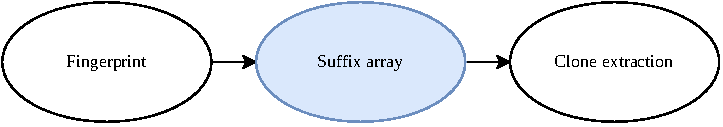
\includegraphics[width=0.8\textwidth]{figures/phases/phases_suffix.drawio.pdf}
    \end{center}
\end{figure}

Now that we know how the fingerprint has changed after an edit, the next phase is to input
the edit operations into an algorithm which dynamically updates the extended suffix array.
The algorithm discussed in this section will be run once for each edit operation.

Constructing/updating the suffix array is the most time-consuming phase of the algorithm,
so the goal for the dynamic update is to take the previous suffix array and an edit
operation, and compute the new suffix array faster building the suffix array from scratch.
We will also in the following section convert the suffix array into a dynamic structure,
which allows insertions, deletions and increments faster than linear time.

The algorithm used is the algorithm presented by Salson et
al.~\cite{DynamicExtendedSuffixArrays}. This algorithm is based on the 4-stage algorithm
for updating a Burrows-Wheeler transform (BWT), also presented by Salson et
al.~\cite{DynamicBWT}. Recall that the BWT is a transform on an input string which is
often used for compression and text-search purposes. The BWT is also reversible by using
the LF function to compute the original string in reverse. The LF function is computed for
a position $i$ such that $LF(i) = rank_{BWT[i]}(i) + C[BWT[i]]$ where the array $C$
contains for any character $c$, how many characters are lexicographically smaller than
$c$. This function can intuitively be used in the context of the BWT to allow us to move
from $CS_i$ to $CS_{i-1}$. Also recall that the suffix array and the BWT of a string is
tightly related to the point where one can compute the BWT from the suffix array. Any
updates to the BWT will also correspond to similar updates to the suffix array, so the
algorithm which updates the BWT can be used to determine how the suffix array changes as
well.

\subsection*{Updating BWT on insertion}

First we will observe which parts of a BWT changes when we insert a single character. Note
that we will only consider changes to the BWT, meaning the final character in each shift,
not the whole cyclic-shift. We will consider an insertion of a character $c$, inserted at
position $i$. We know that we will have exactly one more $CS$ for the string, which starts
with the inserted character $c$, at position $i$. This $CS$ ends with the character at
position $i - 1$. We also know that exactly one $CS$ will change its last character, which
is the cyclic-shift previously starting at position $i$, but is now at position $i + 1$
after the insertion. This new cyclic-shift will now end with the new inserted character,
$c$. These are the only changes that happen to the characters in the BWT, but the ordering
might not be correct anymore.

\begin{table}[t]
	\begin{center}
		\subfloat[S = BANANA\$]{
			\begin{tabular}{c | l}
				Order & Cyclic-shift \\
				\hline
				6     & \$BANAN\textbf{A}   \\
				5     & A\$BANA\textbf{N}   \\
				3     & ANA\$BA\textbf{N}   \\
				1     & ANANA\$\textbf{B}   \\
				0     & BANANA\textbf{\$}   \\
				4     & NA\$BAN\textbf{A}   \\
				2     & NANA\$B\textbf{A}   \\
			\end{tabular}
		}
        \hspace{1cm}
		\subfloat[S = BABNANA\$]{
			\begin{tabular}{c | l}
				Order & Cyclic-shift \\
				\hline
				7     & \$BABNAN\textbf{A}   \\
				6     & A\$BABNA\textbf{N}   \\
				1     & ABNANA\$\textbf{B}   \\
				4     & ANA\$BAB\textbf{N}   \\
				0     & BABNANA\textbf{\$}   \\
				2     & BNANA\$B\textbf{A}   \\
				5     & NA\$BABN\textbf{A}   \\
				3     & NANA\$BA\textbf{B}   \\
			\end{tabular}
		}
		\caption{BWT for string before and after insert}
		\label{table:bwtupdate}
	\end{center}
\end{table}

For the string \verb|BANANA$|, let $c = \verb|B|$, and $i = 2$, which results in the
string \verb|BABNANA$|. In table \ref{table:bwtupdate} we can see that some substrings of
the BWT is preserved, such as \verb|$AA| and \verb|AN|, but some other changes have
occured. In table \ref{table:bwtupdatestages} We see that the new $CS_2$ is
\verb|BNANA$BA|, and the changed $CS_3$ is \verb|NANA$BAB|. We can find where these
cyclic-shifts are located by first looking up $i$ in the ISA, $\ISA{2} = 6$. This is the
location of $CS_3$ (after the insertion), where the final character is updated to the
inserted character \verb|B|. To find the position where the new cyclic-shift should be
inserted, we can use the LF function to move from the $CS_3$ to $CS_2$. Computing
$LF(6)$ after the substitute gives us $5$, which is where the new $CS_2$ should be
inserted in the BWT. When we insert in the BWT, we only need to consider the final
character of $CS_2$, which in this case is \verb|A|, the character which was previously
substituted.

\begin{table}[t]
	\begin{center}
		\subfloat[Original BWT]{
			\begin{tabular}{c | l | l}
				Order & F  & L           \\
				\hline
				6     & \$ & A  \\
				5     & A  & N  \\
				3     & A  & N  \\
				1     & A  & B  \\
				0     & B  & \$ \\
				4     & N  & A  \\
				2     & N  & A  \\
			\end{tabular}
		}
		\hspace{1cm}
		\subfloat[After change and insert]{
			\begin{tabular}{c | l | l l}
				Order & F  & L  \\
				\hline
                7     & \$ & A & \\
				6     & A  & N & \\
				4     & A  & N & \\
				1     & A  & B & \\
                0     & B  & \$& \\
                2     & \textbf{B}  & \textbf{A} & Inserted \\
                5     & B  & A & \\
                3     & \textbf{N}  & \textbf{B} & $A \rightarrow B$ \\
			\end{tabular}
		}
		\hspace{1cm}
		\subfloat[After reordering]{
			\begin{tabular}{c | l | l l}
                Order & F  & L & \\
				\hline
                7     & \$ & A & \\
                6     & A  & N & \\
                1     & \textbf{A}  & \textbf{B} &  \multirow{2}{*}{$\updownarrow$} \\
                4     & \textbf{A}  & \textbf{N} & \\
                0     & B  & \$& \\
                2     & B  & A & \\
                5     & B  & A & \\
                3     & N  & B & \\
			\end{tabular}
		}
		\caption{BWT for string before and after insert}
		\label{table:bwtupdatestages}
	\end{center}
\end{table}


The final stage of the algorithm now that all the elements are present, is to rearrange
the cyclic-shifts which have changed their lexicographical ordering. It is possible that
the cyclic-shifts change their ordering because of the new character. For example
\verb|ANANA$B| $<$ \verb|ANA$BAN|, but \verb|ABNANA$B| $>$ \verb|ANA$BABN|. A useful
observation is that only $CS_j$ where $j \leq i$ will have their lexicographical ordering
changed. This is because only in these cyclic-shifts the inserted \verb|B| comes before
the \verb|$|. Since the \verb|$| is the smallest lexicographical character, and no two
cyclic-shifts will have \verb|$| in the same location, we know that the lexicographical
comparison of two cyclic-shifts will never go past the \verb|$|.

We know that only $CS_j$ where $j \leq i$ can have their ordering changed, and we have
already inserted $CS_i$ at the correct position (the new cyclic-shift). We will store two
positions, $pos$ and $expected$, where $pos$ is initially the position of $CS_{i - 1}$,
which was stored before any changes were made to the BWT. $pos$ is therefore the actual
position of $CS_{i - 1}$, $expected$ is the expected position of $CS_{i - 1}$, which is
computed by computing $LF(insertionPoint)$ where $insertionPoint$ is the position where
the new $CS_i$ was inserted. With the knowledge of where the cyclic-shift of order $i - 1$
is, and where it should be, we can move the cyclic-shift to that position. In the example,
we have that the $expected = 3$, and $pos = LF(5) = 2$ after the insertion gives us the
expected location of the cyclic-shift of order $1$. Therefore, we remove the cyclic-shift
at position $3$, and insert it again at position $2$.

Before performing the row-move, we also compute $newPos = LF(pos)$ which will give us the
position of the cyclic-shift of order $i - 2$. After the row-move, we can continue
comparing the position and expected position by updating $pos = newPos$, and $expected =
LF(expected)$. In the example this would update both $pos$ and $expected$ to $4$. Since
the expected position and actual position is the same, the algorithm is done, and we know
that every position of the BWT is now in the correct location. We know that there will be
no more row-moves for any other $CS$ down to order $0$ because $LF(pos) = LF(expected)$,
which would be true for all future iterations as soon as $pos = expected$

\subsection*{Updating SA on insertion}

The suffix array is updated similarly to the BWT. When we insert the new cyclic-shift at
position $5$ in the BWT, we similarly insert the value $2$ at position $5$ in SA. We
insert the value $2$ because the new suffix which corresponds to the new cyclic-shift
starts at the position where the new character was inserted, which was $2$. When the new
cyclic-shift is inserted, we are now in an invalid state for the suffix array, because we
have two elements with the value $2$. Note that a suffix array is always a permutation of
the values $(0..n)$ where $n$ is the number of characters in the input. Since we have
inserted a new suffix in the suffix array which is the 2nd smallest suffix, all the
previous suffixes which had a value $j \geq 2$ is now incremented. After incrementing all
these suffixes, we are now in a valid suffix array state, but similarly to our BWT, some
suffixes may have had its ordering changed. For every move-row operation in the BWT, the
elements in SA are reordered in the same fashion.

\begin{algorithm}[t]
  \SetAlgoLined\DontPrintSemicolon
    \algo{\UpdateSuffixArrayInsert{SA, ISA, BWT, i, ch}}{
        $\Var{posFirstModified} \gets \ISA{\Var{i}}$ \;
        $\Var{previousCS} \gets \LF{$\Var{BWT}, \Var{i}$}$ \;\;

        $\Var{storedLetter} \gets \ArrayAccess{\Var{BWT}}{\Var{posFirstModified}}$ \;
        $\ArrayAccess{\Var{BWT}}{\Var{posFirstModified}} \gets \Var{ch}$ \;\;

        $\Var{insertionPoint} \gets \LF{$\Var{BWT}, \Var{i}$}$ \;
        \lIf{$\Var{storedLetter} < \Var{ch}$} {
            $\Var{insertionPoint} \gets \Var{insertionPoint} + 1$
        } \;

        \Comment{Insert storedLetter in BWT at pointOfInsertion}
        \Insert{$\Var{BWT}, \Var{insertionPoint}, \Var{storedLetter}$}\;\;
        \Comment{Insert i in SA at pointOfInsertion, increment all values $\geq$ position}
        \Insert{$\Var{SA}, \Var{insertionPoint}, \Var{pos}$}\;
        \IncrementGreaterThan{$\Var{SA}, \Var{pos}$}\;\;


        \lIf{$\Var{insertionPoint} \leq \Var{previousCS}$} {
            $\Var{previousCS} \gets \Var{previousCS} + 1$
        } \;


        $\Var{pos} \gets \Var{previousCS}$ \;
        $\Var{expected} \gets \LF{$\Var{insertionPoint}$}$ 

        \While{$\Var{pos} \neq \Var{expected}$}{

            $\Var{newPos} \gets \LF{$\Var{pos}$}$ \;\;

            \Comment{Delete value at pos and reinsert at expected in BWT and SA}
            \MoveRow{$\Var{pos}, \Var{expected}$} \;\;

            $\Var{pos} \gets \Var{newPos}$ \;
            $\Var{expected} \gets \LF{$\Var{expected}$}$ \;

        }
    }

  \vspace{0.5cm}
  \caption{Update BWT and suffix array when inserting a single character}
  \label{alg:updatesuffixarrayinsert}
\end{algorithm}

Algorithm \ref{alg:updatesuffixarrayinsert} dynamically updates a suffix array and BWT
when a single character is inserted. This algorithm can easily be extended to insert a
string instead of a single character by adding a loop which continuously updates the
\verb|pointOfInsertion| to the previous $CS$ with the LF function, and inserts all the
characters at that position into the BWT and SA backwards. This is more efficient than
calling the single character algorithm multiple times, because the reordering stage is
only performed once. The details for insertions/deletions of multiple characters is
covered in the original paper~\cite{DynamicExtendedSuffixArrays}.

\subsection*{Deletion}

A deletion of a single character is a similar procedure as an insertion, as it is simply
reversing the substitution and insertion, and then performing the reordering stage again.
If we have the string \verb|BABNANA$|, and delete the \verb|B| at position $2$, We know
that there will be exactly one $CS$ removed. This is $CS_2$ which starts with the deleted
character \verb|B|, and ends with the character before it, \verb|A|. There is also a
single $CS$ which will have its final character changed, $CS_3$, because the final
character \verb|B| will be deleted. The final step is to again perform the reordering
stage for $CS_j$ where $j \leq 2$, as these are the only cyclic-shifts which can have
their lexicographical ordering changed.

The algorithm which performs the deletion at position $i$ will do the deletion and
substitution in the opposite order. First we find both the $CS$ which will have its
character substituted in the BWT, and the $CS$ which will have its character deleted in
the BWT. The character to be substituted will be found with $substituted = ISA[i + 1]$,
and the character to delete will be found with $deleted = LF(substituted)$. $BWT[deleted]$
is then deleted, and $BWT[substituted]$ is substituted with the character that was
deleted. Finally, the reordering phase is performed in the same fashion, where $pos$ is
set to the position of the original $CS_{i - 1}$ and $expected$ is set to $LF(substituted)$

In our example $substituted = ISA[3] = 7$, $deleted = LF(7) = 5$ and $pos = LF(5) = 2$.
Then $BWT[deleted]$ is deleted, and $BWT[substituted]$ is set to the deleted character.
Then $expected = LF(6) = 3$. Note that $substituted$ was decremented after the deletion
because the deletion moved that $CS$ one position up. When the reordering stage happens,
we have $pos = 2$ and $expected = 3$, so we perform the reordering in the BWT and SA in the
same fashion as previously, and the algorithm will again terminate after one iteration of
the reordering phase.

\subsection*{Substitution}

Substitution operations are also possible and covered in the original paper, but in
CCDetect-LSP these were simply implemented as a deletion followed by an insertion. This is
less efficient than a single operation, since the reordering stage is done twice, but we
do not suspect that this will worsen the performance in any significant way.

\subsection*{LF function}

The LF function is called multiple times for any operation which is done to update the
suffix array. Therefore, it is important to be able to efficient compute $LF$ at any point
in time. The naive approach of linearly iterating through the BWT to compute the $rank$
and number of smaller characters is too slow. Recall that $LF(i) = rank_{BWT[i]}(i) +
C[BWT[i]]$ where $rank_{BWT[i]}(i)$ is the rank for the character $BWT[i]$ at position $i$
in the BWT, and $C[BWT[i]]$ counts the number of lexicographically smaller characters than
$BWT[i]$ in the BWT. We therefore need a data structure for $rank$ queries on the BWT, and
a data structure which stores the number of smaller characters of each character in the
BWT. 

For the $rank$ queries, recall that the wavelet matrix was a data structure which could
efficiently compute $rank/select$ queries for strings. We will use the wavelet matrix to
store the BWT and perform efficient $access$ and $rank$ queries on it as needed. With the
wavelet matrix, we do not need to store the BWT itself, as we can simply query the wavelet
matrix to access characters of the BWT. We also do not need to store the full fingerprint,
since we can access characters in the wavelet matrix and if we need to access the
characters in a sorted order, we can use the LF function. We decided to use the wavelet
matrix instead of a wavelet tree as it has been shown to have faster $rank$ queries, and
is more memory efficient for larger alphabets. Our alphabet can be quite large compared
the standard applications of $rank/select$ data structures (such as DNA analysis). The
wavelet matrix is also generally simpler to implement, and can be dynamically updated in a
simple manner. Each bitset in the wavelet matrix is a dynamic bitset where we can
efficiently insert and delete characters as needed when the size of the BWT grows/shrinks.

When inserting a character $c$ into the wavelet matrix at position $i$, we insert the
first bit of $c$ in level $0$ in the matrix at position $i$. The next bit of $c$ is then
inserted in level $1$ in the matrix at position $rank_x(WM[0], i)$ where $x$ is the value
of the previous bit.

A complication with the wavelet data structures is to update the data structure as the
alphabet increases in size. In our case the alphabet size will at some point increase to a
size where elements need an additional bit. For the wavelet matrix, this can be solved by
simply inserting a new row at the beginning of the matrix (level $0$), where the bitset
consists of all zeroes. Afterwards, the new element is inserted in the normal fashion,
which should be the only element with a $1$ bit in the first position.

\Todo{Algorithm to insert/delete in wavelet matrix}

The $C$ array can be implemented in two ways. Either $C[c]$ holds the number of smaller
character than $c$ in the input, or $C[c]$ holds the number of occurrences of $c$. There
are trade-offs with either implementation, as storing the number of smaller characters
requires a linear scan whenever a character is inserted/deleted, while storing the number
of occurrences requires computing the number of characters whenever the LF function is
called. We have chosen the approach of storing the number of occurrences, as updating the
array is simpler in cases where the alphabet size increases. When we later update LCP
values, we will see that there is a possibility that choosing the option of storing the
number of smaller characters in $C$ is faster. 

\section{Dynamic extended suffix arrays}

A major bottleneck when inserting/deleting elements in the suffix array is that when an
element is removed, all elements after it needs to be moved by one index so that the gap
is closed. This is also the case in the reordering stage, where all the elements between
the old position and new position of an element needs to be moved by one position. In
addition, since a suffix array is always a permutation from $0$ to $n$ where $n$ is the
number of elements in the input, we need increment/decrement all elements greater than or
equal to the element which was inserted/deleted. For example, if we insert a new element
into the suffix array which indicates that a new suffix is the ith smallest, then
naturally the previous suffix with value $i$ in SA should now have the value $i + 1$,
which applies to all other suffixes lexicographically greater than the new suffix as well.
In a standard representation for a suffix array (an array), this would require either a
linear scan through the entire SA, or a linear scan through ISA from position $i$, which
is also linear in the worst case. Multiple linear scans through the SA would make the
algorithm slower than the linear time SACA when the amount of inserted/deleted character
increases. 

In this section we will introduce a data structure called the dynamic extended suffix
array. This data structure consists of a dynamic permutation, which facilitates
insertion/deletion of elements in a permutation from $0$ to $n$, without linear scans to
close gaps or incrementing/decrementing elements. The data structure stores SA, ISA and
LCP and is inspired by the data structure introduced for the same purpose by Salson et
al.~\cite{DynamicExtendedSuffixArrays}. The data structure used by Salson et al. uses the
same dynamic permutation tree, but reduces the amount of values which is stored to reduce
memory consumption, but also slows down the access time of elements in the permutation.
Our data structure will not be compressed, which allows faster access to arbitrary
elements, and will be extended to also include the LCP values as well. Therefore, this
data structure encompasses the entire extended suffix array.

The data structure consists of two balanced binary trees, with pointers between elements
in one tree to the other. Figure \ref{fig:dynamicpermutation} shows the two trees
which are labeled the $A$ tree and the $B$ tree. Note that the trees do not actually hold
the values displayed in the figure, the values in each node of the figure only represents
the inorder position of each node, which is called the inorder rank of the node.

To construct a permutation such as $[6,5,3,1,0,4,2]$, for each element, insert a node in
each tree. After the trees have all the nodes in them, pointers are added from a node in
$A$ to a node in $B$ and vice versa (doubly linked). If an element in SA has a value $i$
at position $j$, pointers will be added between the node in $A$ with inorder rank $i$, and
the node in $B$ with inorder rank $j$. 

Now the tree is complete, but we can also insert new nodes into the data structure as the
suffix array grows. When a new value $j$ is added at position $i$, a node is inserted into
$A$ such that it has the inorder rank of $i$, and a node is inserted into $B$ such that it
has the inorder rank of $j$. For example if we wanted to insert a new value $4$ at
position $1$ in the permutation in figure \ref{fig:dynamicpermutation}, we would insert a
new node in $A$ so that it is the right child of the node labeled $0$, and then insert a
new node in $B$ which is the left child of the node labeled $4$. The trees can intuitively
be understood such that the inorder values in $A$ represent the indices of the
permutation, and the inorder values in $B$ represent the values in the permutation.
Therefore, if we look at a node in $A$ with inorder rank $i$, and follow the pointer to a
node in $B$ with inorder rank $j$, this means that the permutation has the value $j$ at
position $i$. 

Deleting a node at position $i$ is similar, but we will instead find the node with a rank
of $i$ in $A$, then delete that node and the node it points to in $B$. As the trees are
implemented as balanced trees, traversing, inserting and deleting nodes takes $O(\log n)$

An essential property of this tree is that when a new value $j$ is inserted into the
permutation at position $i$, all indices $\geq i$ and values $\geq j$ is incremented by
$1$. This is because all the nodes which had an inorder rank greater than or equal to the
new nodes in each respective tree has now been incremented by $1$ simply because the
structure of the tree has changed. No additional work is required to increment the
elements. 

The part we are still missing is how to find a node with inorder value $i$, and how to
determine the inorder value of a given node. We cannot afford to traverse all the nodes in
an inorder fashion to find a node with a specific inorder rank. Therefore, the trees are
implemented as order-statistic trees~\cite[340]{CLRS}. An order-statistic tree is a tree
where each node $x$ stores an additional integer $size$, which contains the number of
nodes in the subtree rooted at $x$. This allows us to easily determine how many nodes is
in the left subtree of a given node, and use this to determine where the node with a
certain inorder rank is located. If we wanted to find the node in the $A$ tree of figure
\ref{fig:dynamicpermutation} with inorder rank $4$, we would start at the root, see that
the left subtree of the root contains $3$ nodes. Therefore, the roots inorder rank is $3$.
With this information we know that we need to traverse to the right child, and look for
the node with inorder rank $4 - 4 = 0$ in that subtree (since we have already seen 4
nodes). Since the node labelled $5$ has a rank of $1$ (in its own subtree), we know to
traverse left, and at that point we have reached the correct node.

\begin{figure}[t]
	\begin{center}
		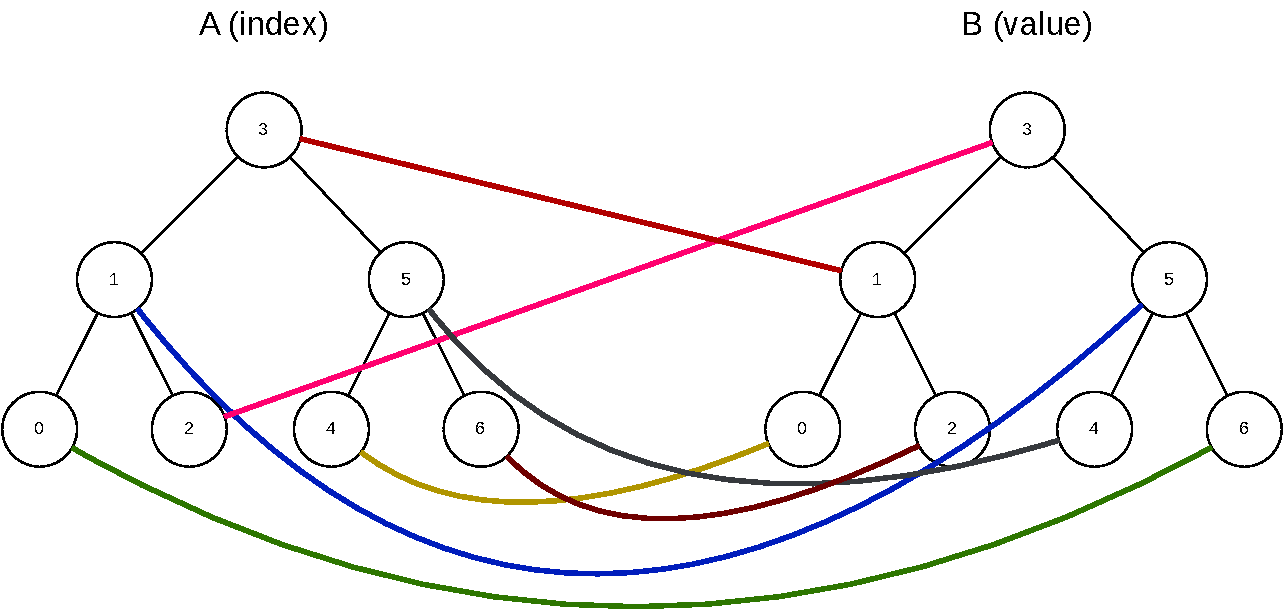
\includegraphics[width=0.95\textwidth]{figures/dynamicpermutation.drawio.pdf}
	\end{center}
	\caption{Dynamic permutation for the permutation $[6,5,3,1,0,4,2]$. Colors have no meaning except to make lines clearer}
	\label{fig:dynamicpermutation}
\end{figure}

\begin{algorithm}[t]
  \SetAlgoLined\DontPrintSemicolon
    \algo{\GetNodeByRank{root, rank}}{
        $\Var{current} \gets \Var{root}$ \;

        \While{$\Var{current} \neq \Null$}{
            $\Var{currentRank} \gets \Access{\Access{\Var{current}}{\Var{left}}}{\Var{size}}$

            \uIf{$\Var{currentRank} = \Var{rank}$}{
                \Break \;
            }
            \uElseIf{$\Var{currentRank} > \Var{rank}$}{
                $\Var{current} \gets \Access{\Var{current}}{\Var{left}}$
            }
            \Else{
                $\Var{current} \gets \Access{\Var{current}}{\Var{right}}$ \;
                $\Var{rank} \gets \Var{rank} - \Var{currentRank} + 1$
            }
        }
        \Return $\Var{current}$
    }

  \vspace{0.5cm}
  \caption{Find the node in a tree with a given inorder rank}
  \label{alg:getnodebyrank}
\end{algorithm}

\begin{algorithm}[t]
  \SetAlgoLined\DontPrintSemicolon
    \algo{\GetRankOfNode{node}}{
        $\Var{rank} \gets \Access{\Access{\Var{node}}{\Var{left}}}{\Var{size}}$ \;
        \While{$\Access{\Var{node}}{\Var{parent}} \neq \Null$}{
            \If{$\Access{\Access{\Var{node}}{\Var{parent}}}{\Var{right}} = \Var{node}$}{
                $\Var{rank} \gets \Var{rank} + \Access{\Access{\Var{node}}{\Var{parent}}}{\Var{right}} + 1$
            }
            $\Var{node} \gets \Access{\Var{node}}{\Var{parent}}$
        }

        \Return $\Var{rank}$
    }

  \vspace{0.5cm}
  \caption{Find the inorder rank of a given node}
  \label{alg:getrankofnode}
\end{algorithm}

Algorithm \ref{alg:getnodebyrank} shows how to find a node in a tree by its inorder rank,
and algorithm \ref{alg:getrankofnode} shows how to determine the rank of a given node. The
algorithm to find the value at a certain position is simple with these algorithms. To find
the value in the permutation at position $i$, find the node with inorder rank $i$ in $A$,
follow its pointer to a node in $B$, and then find the inorder rank of that node, which is
the value at position $i$ in the permutation. We can also find the position of any value
$j$ in the permutation by performing this algorithm in reverse, by instead starting at the
$B$ tree, finding a node with rank $j$, then following its pointer to a node in $A$ and
returning that nodes inorder rank.

\begin{algorithm}[t]
  \SetAlgoLined\DontPrintSemicolon
    \algo{\DynamicPermutationAccess{permutation, i}}{
        $\Var{aNode} =
        \GetNodeByRank{$\Access{\Access{\Var{permutation}}{\Var{A}}}{\Var{root}}, \Var{i}$}$ \;
        $\Var{bNode} = \Access{\Var{aNode}}{\Var{pointer}}$

        \Return \GetRankOfNode{$\Var{bNode}$}
    }

  \vspace{0.5cm}
  \caption{Get value at position $i$ in a permutation}
  \label{alg:dynamicpermutationaccess}
\end{algorithm}

With the ability to both find a value at a given position in the permutation, and also
finding the position of a given value, we can use this data structure to represent the
suffix array and inverse suffix array, instead of a simple array. Inserting, deleting and
accessing a node in this data structure takes $O(\log n)$ time, and we no longer need a
linear scan through the data structure to increment/decrement values, as values are
automatically incremented/decremented when a new element is inserted/deleted.

\section{Dynamic LCP array updates}

Now that we have a dynamic structure to represent SA and ISA, we can extend the data
structure to also contain the LCP array, and efficiently update the LCP values as well.

Since every node in the $A$ tree of our data structure correlates to an index, we can
easily extend the data structure to contain LCP values by setting a value in each node of
the $A$ tree. This would make the $A$ tree work as a balanced binary tree for the LCP
values, and if an SA value at position $i$ is deleted, the LCP value stored in
the respective node is also deleted.

In the initial construction of the dynamic permutation, LCP values would be inserted
together with the nodes. When dynamically updating the LCP values as suffixes are
inserted/removed, the procedure is more complicated. Salson et
al.\cite{DynamicExtendedSuffixArrays} also describe a procedure for updating the LCP
values after an insert/delete operation, which we will use.

When inserting a character into the input string, the suffix array changes by inserting a
new value, and afterwards moving values from one position to another (reordering stage).
Similarly, a deletion in the suffix array consists of deleting a value, and performing the
same reordering operations. The moving of a value from position $i$ to $j$ can be
decomposed into a deletion at position $i$ followed by an insertion at position $j$. When
updating the LCP array we therefore need to consider how insertion of a value and deletion
of a value in SA affects the LCP values.

The idea for this algorithm is to keep track of all positions which could possibly have
its LCP value changed, and update the LCP values after the SA is fully updated. There are
four different cases where an LCP value at a position $i$ could be changed:

\begin{enumerate}
    \item A suffix was inserted at position $i - 1$ in SA, which is the new suffix that
        the suffix at position $i$ should compute its LCP value for.

    \item The suffix at position $i - 1$ was deleted in SA, making the suffix at position
        $i - 2$ the new suffix that the suffix at position $i$ should compute its LCP
        value for.

    \item A character was inserted/deleted in the middle of the LCP for the suffix at
        position $i$ in SA, which shortens the LCP value between it and the suffix at
        position $i - 1$, and the LCP value between the suffix at position $i$ and $i + 1$.

    \item A character was inserted/deleted at the end of the LCP for the suffix at
        position $i$ in SA, which could potentially extend the LCP value between it and
        the suffix at position $i - 1$, and the LCP value between the suffix at position
        $i$ and $i + 1$.

\end{enumerate}

To cover the first two cases, we will store a dynamic bitset where a set bit at position
$i$ indicates that at some point, the LCP value at position $i$ needs to be updated.

For an insertion at position $i - 1$ in SA (case 1), we will set the bit at position $i$,
as the suffix it compares its LCP to has changed. We will also insert a set bit at
position $i - 1$, as the newly inserted suffix also needs to compute its LCP value with
the suffix at position $i - 2$.

Similarly, for a deletion at position $i - 1$ in SA (case 2), we will set the bit at
position $i$, as the suffix it used to compare its LCP to has been deleted. We will also
delete the bit at position $i - 1$, as the suffix at that position has been deleted.

After setting these bits while performing an insert/delete operation in the SA, the bitset
now contains all the positions of LCP values which need to be updated for the first two
cases. The other two cases are more complex to find the positions of. Instead of inserting
the positions of these suffix into the bitset, we will iterate over the suffixes which
could possibly have their LCP value changed. Iteration over every suffix and recomputing
the LCP value takes linear time in the size of the fingerprint and is therefore too slow
for this algorithm. However, we can reduce the number of suffixes we need to update by
using a series of observations.

The first observation is that we only need to consider suffixes where the
insertion/deletion of a character at position $i$ has changed the suffix. Those are the
suffixes which start at a position $j$ where $j \leq i$. Other suffixes cannot change, as
the insertion/deletion happened before the starting position of the suffix. For a suffix
at position $j$ which has changed, two LCP values can change, the values at position $k$
and $k + 1$ where $SA[k] = j$. These two LCP values can change, because at position $k$,
the suffix at position $SA[k]$ is compared with $SA[k - 1]$, and at position $k + 1$, the
suffix at position $SA[k + 1]$ is compared with $SA[k]$. Since both of these LCP values
depend on the suffix at position $SA[k] = j$, they can potentially change when the suffix
is changed. The positions in SA which possibly can be changed can be found using the
LF function. In the final phase of the suffix array update algorithm when we have
inserted/deleted an element at position $i$, we are reordering suffixes at position $j
\leq i$. These are the suffixes we are looking for, but we can skip all suffixes which are
reordered, as they are already marked to be computed in the bitset for the previous cases.
Therefore, the variable $pos$ points to the next suffix we need to consider at the end of
algorithm \ref{alg:updatesuffixarrayinsert}.

Another useful observation when iterating over suffixes is that after an
insertion/deletion, no two suffixes will have the insertion/deletion occur at the same
position. This is true because no two suffixes start on the same position in the input,
and an insertion/deletion at a position $i$ in the input can therefore never correspond to
an insert/deletion at the same position for two different suffixes. With that in mind,
another useful observation is that given two suffixes with an LCP value of $p$, any change
inside the range of the LCP in either of the suffixes, will change $p$.

The idea is to determine if the insertion/deletion is out of range to possibly affect the
LCP value of a suffix. Recall that the LCP value for a suffix at position $i - 1$ is at
minimum one less than the LCP value for the previous suffix at position $i$, as discussed
in \cref{initialdetection}. We can determine that it is impossible for the LCP value at
position $i - 1$ to change, if neither of the LCP values which is affected by the suffix
at position $i$ changes, unless the insertion/deletion happens at position $i - 1$. This
is explained by the fact that at minimum, the LCP of the suffix at position $i$ covers
every character of the LCP of the suffix at position $i - 1$ except for the first
character. If the first character was the position of the insertion/deletion, it can
change the LCP value, but that case is already handled by the positions stored in the
bitset. Since the suffix at position $i - 1$ did not update, this holds recursively for
the next suffix at position $i - 2$ as well. Therefore, as soon as we find a single suffix
at position $i$ which does not lead to an LCP value update, this will recursively hold for
all suffixes at position $j < i$.

With this in mind, the algorithm to update the LCP array has two stages. Given the bitset
of positions which need to be updated in correlation with the first two cases, we perform
a $select$ operation to continuously find the location of set bits in the bitset, and use
their position to determine which positions in the LCP array need to be computed. After
all the positions in the bitset has been updated in the LCP array, we move on the last two
cases. From the position of $pos$, which was computed during the suffix array update, we
continuously call the LF function on $pos$ to find the previous suffix. At each position,
we update the LCP value of the suffix at position $pos$ and $pos + 1$, as these two LCP
values are both affected by the suffix at position $SA[pos]$. When we encounter the
situation where both LCP values at position $pos$ and $pos + 1$ did not lead to a change
in LCP values, the algorithm is finished and the LCP array is updated. Algorithm \ref{}
shows how the LCP array is updated, given the bitset of updated positions which is built
during algorithm \ref{alg:updatesuffixarrayinsert}.

The actual computation of LCP values is also more complex than it seems. In the dynamic
detection algorithm we are not storing the entire fingerprint, we only have the BWT stored
in the wavelet matrix, and the LF function allows us to move from one character to the
previous in the original input text. When we compute LCP values, we need to be able to
compare characters in two suffixes from start to potentially end of the input, therefore
we need to be able to move from one character to the next, which is the inverse of the LF
function. 

The inverse LF function for a position $i$ computes the next cyclic-shift by first
determining what character is in the first column of the CS at position $i$ in the sorted
cyclic-shifts, and its $rank$ in the first column. With the character and rank of that
character, we can perform a $select$ on the BWT for that character and rank, which will
give us the location of where that character is located in the last column (BWT) which is
the next CS. This is the next cyclic-shift because it is the cyclic-shift where the
character which was previously in the first column, but is now cycled one character to the
left, which corresponds to the next CS. To find which character is in the first column at
position $i$, recall that the $F$ column in the sorted cyclic-shifts just contain all the
characters of the input in sorted order. We can therefore use the $C$ to determine which
character is located at exactly position $i$, just by counting the number of occurrences
of the previous characters. If $C$ is instead implemented as an array where the $C[c]$
holds the number of smaller characters than $c$ in the input, finding the correct
character can be done efficiently with a binary search. When we know which character is
located at position $i$ in the first column, we do $select_c(i - C[c])$ to determine where
that occurence of $c$ is located in the last column (the BWT), which is then returned as
the result of the inverse LF function.

With the inverse LF function, computing the LCP value between two suffixes at position $i$
and $j$ is done by repeatedly applying the inverse LF function to $i$ and $j$, and
comparing the characters at those positions in the BWT.

\Todo{Algorithm for iterating over suffixes which need to update their LCP value}

\Todo{Algorithm for updating a single LCP value}

\section{Dynamic clone extraction and source-mapping}

\begin{figure}[H]
    \begin{center}
        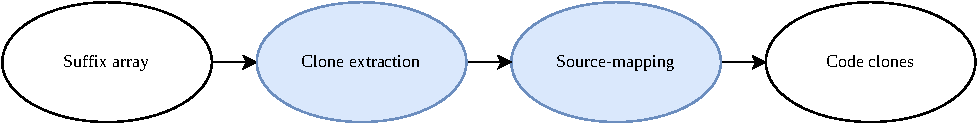
\includegraphics[width=1\textwidth]{figures/phases/phases_extractionandsourcemap.drawio.pdf}
    \end{center}
\end{figure}

The LCP is no longer represented as an array, but as a a balanced tree. As trees are more
costly to traverse linearly compared to arrays, we also want to improve how we extract
clones in this phase. The goal of this phase is still to find the indices in the
fingerprint which corresponds to the start of code clones, which will later be mapped back
to the original source code again.

Recall that the algorithm in the initial detection in \cref{initialdetection} traversed
the suffixes from beginning to end, and extracts indices of suffixes where the LCP value
is above the token threshold parameter. Also recall that some clones were filtered, those
being clones which extend past a single fragment, or clones which are contained inside a
larger clone. This algorithm will now be converted to run on the balanced tree which
contains the LCP values, which also optimizes the algorithm to reduce the amount of LCP
values we need to examine.

When updating a value in the LCP array, we can check to see if the new value is above the
token threshold. If the previous value was below the treshold, and the new value is above
the treshold, we know that this is a node which could potentially be a code clone, so
storing these nodes can reduce the amount of nodes we need to examine. Since potentially
multiple updates to an LCP value happens as potentially multiple edit operations are
performed before extracting clone indices, we can reduce the amount of insertions/removals
from this set by filtering nodes with a too low LCP value after we have done all LCP value
updates.

After all LCP values are updated and we have filtered out nodes, we are left with a set of
all the nodes with an LCP value above the token threshold parameter. In order to filter
out clones which are contained within other clones, we need to add a similar check to the
loop which was added in algorithm \ref{alg:cloneextraction}, however since the set only
contains nodes with an LCP values above the token threshold, the algorithm will be
slightly different. Instead of adding a loop which skips past indices which are contained
clones, we can instead check if the last index added contains the current clone we are
looking at. Doing the process in this fashion allows us to skip over many checks if there
are long stretches of suffixes in the fingerprint with LCP values below the token
treshold. Algorithm \ref{alg:dynamiccloneextraction} shows how this algorithm is
implemented.

\begin{algorithm}[t]
  \SetAlgoLined\DontPrintSemicolon
    \algo{\DynamicCloneExtraction{nodesAboveTreshold}}{
        $\Var{clones} \gets \textrm{empty\ list}$

        $\Var{lastAdded} \gets -1$ \;
        $\Var{lastLCP} \gets -1$ \;

        \For{$\Var{node} \In \Var{nodesAboveTreshold}$}{
            
            $\Var{index} \gets \GetRankOfNode{$\Access{\Var{node}}{\Var{pointer}}$}$ \;

            \If{$\Var{lastAdded} \neq -1$}{
                $\Var{difference} \gets \Var{index} - \Var{lastAdded}$ \;
                \If{$\Access{\Var{node}}{\Var{key}} + \Var{difference} \leq \Var{lastLCP}$}{
                    \Continue
                }
            }

            \Add{$\Var{clones}, \Var{node}$} \;
            $\Var{lastAdded} \gets \Var{index}$ \;
            $\Var{lastLCP} \gets \Access{\Var{node}}{\Var{key}}$
        }

        \Return $\Var{clones}$
    }

  \vspace{0.5cm}
  \caption{Extract clone indices in dynamic extended suffix array}
  \label{alg:dynamiccloneextraction}
\end{algorithm}

After applying this algorithm we are left with the nodes with inorder ranks which
correspond to the same indices as in the initial detection, and for the final phase,
mapping the clone indices back to the original source code, we can do almost the same
procedure as in the initial detection. The algorithm for this is almost the same as
algorithm \ref{alg:buildclonemap}, but some parts are changed to avoid traversing through
the trees many times to find the second index, which we would have to do if we used
algorithm \ref{alg:buildclonemap} without any modifications. The problem with algorithm
\ref{alg:buildclonemap} is that it computes the expression $\SA{\ISA{\Var{firstIndex}} -
1}$ to find the index of the matching clone. This is not a problem in the initial
detection, because SA and ISA are arrays, which give $O(1)$ time access. This is not the
case for the dynamic extended suffix array, which would require $O(\log n)$ access time
for that expression. Instead, only the nodes of the clone indices in algorithm
\ref{alg:dynamiccloneextraction} is stored, and for a node $firstNode$, when we can find
the node of the matching $secondNode$ in $O(1)$ time by finding the predecessor of
$\Var{firstNode}$ and following its pointer. Remember that the nodes we have stored as
clone indices are nodes in the $A$ tree which corresponds to $SA$ indices. Following the
pointer corresponds to SA values, or alternatively, ISA indices. After we have both the
$\Var{firstNode}$ and $\Var{secondNode}$, we can get their fingerprint indices by getting
the inorder rank of their pointer, with algorithm \ref{alg:getrankofnode}. Afterwards, the
algorithm continues as previously. While this still requires traversing the tree in
$O(\log n)$ time, we have reduced the number of traversals needed from $5$ with a direct
translation of \ref{alg:buildclonemap} to $2$ with the smarter traversal of nodes
described here.

Now that we have successfully source-mapped from our dynamic extended suffix arrays to
code clones, we are finished, and clones are sent to be displayed to the client.
